\section{Computation of Congruent Numbers}
There are three essentially three computations which I have done.
\begin{enumerate}
  \item The first is brute force computation of congruent numbers using the Pythagoras triplet method discussed in \cref{thm:cong_gen}.
  \item The second is generating the congruent numbers assuming that the BSD conjecture (and hence the converse in Tunnell's theorem) holds true.
  \item The distribution of congruent numbers assuming the BSD conjecture.
\end{enumerate}
\subsection{Brute force Method}
In this method I first generate pairs $(a,b)$ such that $\gcd(a,b) = 1$ and $a+b$ is odd and for each pair the right angle triangle and its area is calculated and added to a list of dictionaries. This is done by the following snippet:
\lstinputlisting[language = Python, firstline = 8, lastline = 20]{code/check_cong.py}
To generate the list of square free congruent numbers I add the "area" key in the dictionary to a set, after removing the square part from the integer. 
\lstinputlisting[language = Python, firstline = 35, lastline = 42]{code/check_cong.py}
This method gives the following output when $N = 40$.
\lstinputlisting{code/bruteforce.txt}
As evident this method is very inefficient to generate congruent numbers. For example the number $13$, which is congruent, has not appeared in this list yet even after $40$ trials.

\subsection{Tunnell's method}
In this method we assume that the BSD conjecture is true and use the converse of Tunnell's theorem to generate a list by checking if each integer below some $N$ is congruent or not. This gives an exhaustive list congruent numbers below $N$. This is much better than the previous method which just gives us $N$ congruent numbers.
\lstinputlisting[language = Python, firstline = 44, lastline = 77]{code/check_cong.py}
Here are all the square free congruent numbers less than $1000$:
\lstinputlisting{code/tunnell.txt}

\subsection{Distribution of square free congruent numbers}
I wrote a method that counts the number of square free congruent numbers less than $N$ using Tunnell's method (assuming the BSD conjecture) and I have plotted their ratio against $N$.
\lstinputlisting[language = Python, firstline = 83, lastline = 92]{code/check_cong.py}
\begin{figure}
  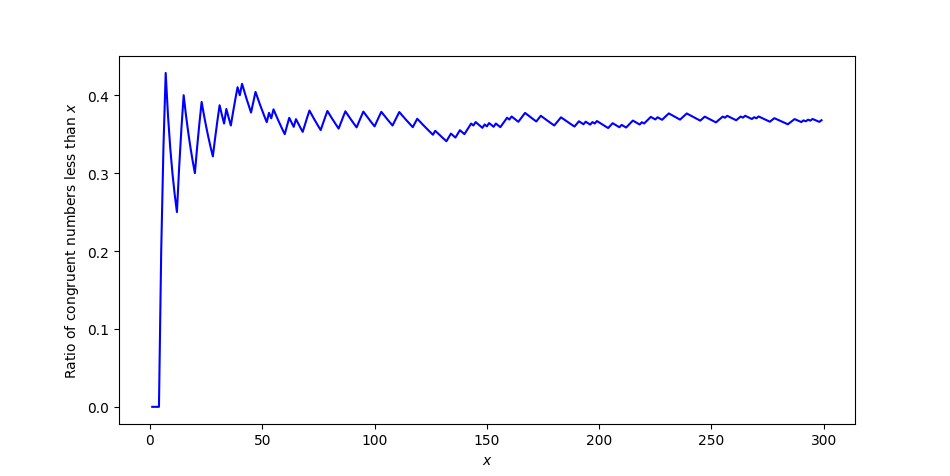
\includegraphics[width = \textwidth]{code/distribution2.png}
  \caption{The distribution for $N = 500$. As observed here this ratio eventually becomes a constant with value of about $0.368$.}
\end{figure}
From the above figure one can also claim the following conjecture.
\begin{conjecture}
  For large enough $n$ the number of square free congruent numbers, $C(n)$, less than $n$ can be approximated by
  \begin{align*}
    C(n) \sim \a n
  \end{align*}
  where $\a \approx 0.368$.
\end{conjecture}
This conjecture will be true given the assumption of the BSD conjecture.
